\documentclass[a4paper, openany]{memoir}

\usepackage[utf8]{inputenc}
\usepackage[T1]{fontenc} 
\usepackage[english]{babel}
\usepackage{amsmath}
\usepackage{amssymb}

\usepackage{booktabs}
\usepackage{fancyhdr}
\usepackage{float}
\usepackage{indentfirst}
\usepackage{graphicx}
\usepackage[linewidth=1pt]{mdframed}
\usepackage{multicol}
\usepackage{fancyvrb}

\usepackage{longtable}

\pagestyle{fancy}
\fancyhf{}
\fancyhead[LE]{\leftmark}
\fancyhead[RO]{\rightmark}
\fancyhead[RE, LO]{PSD}
\fancyfoot[LE, RO]{\thepage}
\fancyfoot[RE, LO]{Pete Gautam}

\renewcommand{\headrulewidth}{1.5pt}

\setcounter{chapter}{17}
\chapterstyle{thatcher}

\begin{document}
\chapter{Startup growth engineering}
Growth engineering builds techniques for systematically introducing a new product idea into a large-scale market and driving it to scale. While a lot of products do fail because they are not desirable, many others fail even though they seem to be desirable. 

Often, some products rise very rapidly and collapse equally fast after a bit of time. Growth engineering gives insight as to why this happens and how we can avoid this.

The challenges in producing a good quality product without defects is still present in startup. But, it also has a bunch of new challenges:
\begin{itemize}
    \item The idea may be new. In such a case, it is difficult to ask the customers what they want precisely. Their advice will not be reliable.
    \item There might not be any customers yet.
    \item The product may be added to a new market.
\end{itemize}

\section{Compounding Growth}
A product experiences compounding growth when the rate of growth is proportional to the number of users. So, the more the number of users, the faster the product grows. This is a very desirable state. 
Growth engineering creates and exploits compounding growth curves. We do this in a very systematic way. A general template of a compounding loop is given below.
\begin{figure}[H]
    \centering
    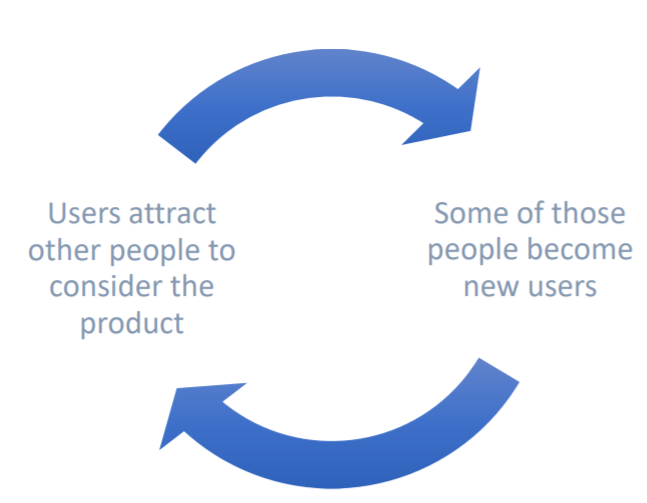
\includegraphics[scale=0.5]{src/18.1 Generic growth loop.PNG}
\end{figure}
\noindent This is the fundamental mechanism behind compounding growth. Current users of the software attract others to use the product. Some of the people do become new users, who then further attract others. This loop continues on an on. The rate of growth is clearly proportional to the number of users- as the number of users grows, the number of people they attract increases. 

The example above shows a direct invitational loop. A specific example of this is given below for WhatsApp.
\begin{figure}[H]
    \centering
    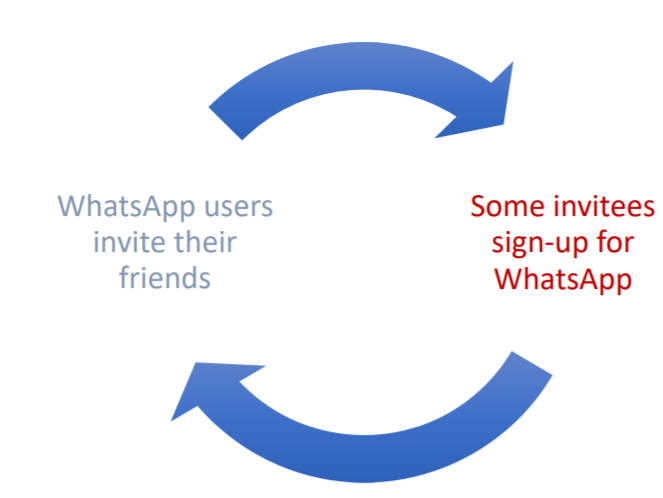
\includegraphics[scale=0.5]{src/18.2 Watsapp growth loop.PNG}
\end{figure}
\noindent WhatsApp users invite their friends, and some of these friends become WhatsApp users. In WhatsApp, it is only possible to chat with those who are already WhatsApp users, so this is a very successful loop.

The following is the direct invitational loop for LinkedIn.
\begin{figure}[H]
    \centering
    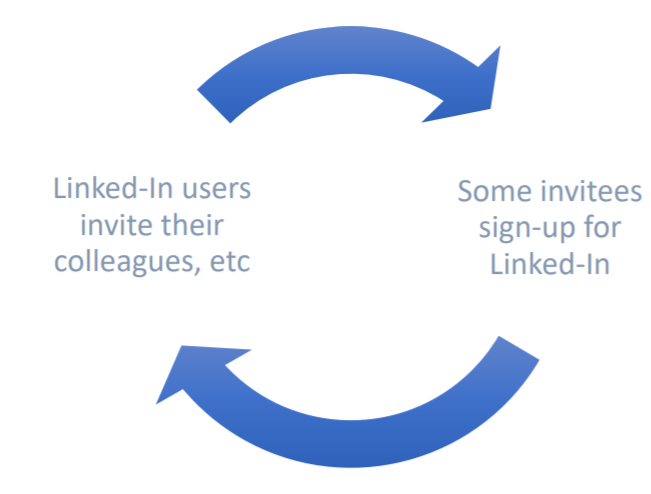
\includegraphics[scale=0.5]{src/18.3 Linkedin growth loop.PNG}
\end{figure}
\noindent LinkedIn users invite their colleages, and some of them become LinkedIn users. LinkedIn has other loops as well, such as a content-driven loop.
\begin{figure}[H]
    \centering
    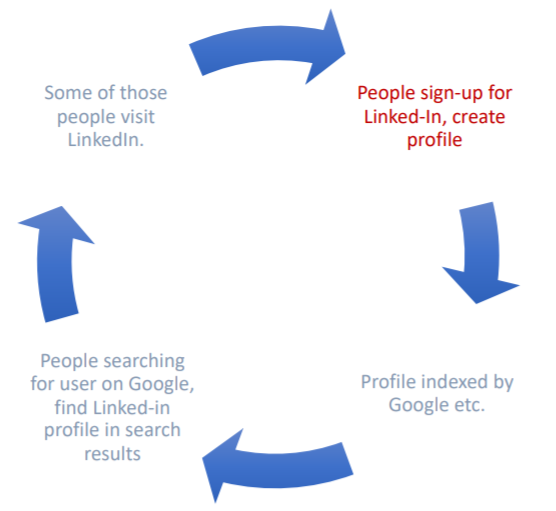
\includegraphics[scale=0.5]{src/18.4 LinkedIn growth loop 2.PNG}
\end{figure}
\noindent A content-driven loop is based on the content that users post. We say that content is the currency of a content-driven loop. A direct-invitation loop uses users as the currency of the loop. This content-driven loop is based on searching profiles/CVs. LinkedIn has a further content-driven loop based on blogs.
\begin{figure}[H]
    \centering
    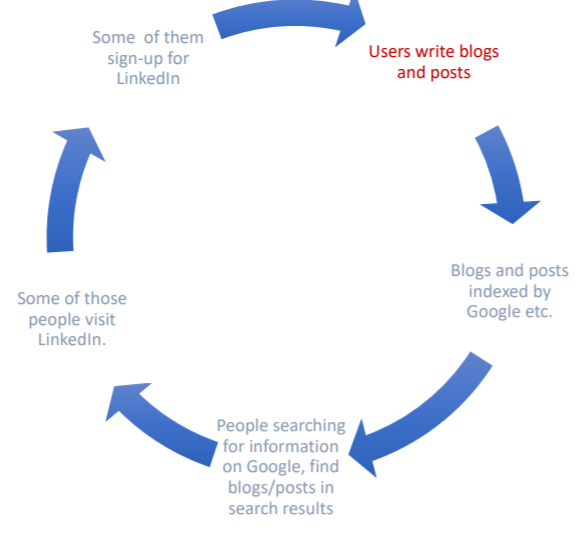
\includegraphics[scale=0.5]{src/18.5 Linkedin growth loop 3.PNG}
\end{figure}
\noindent LinkedIn has other loops as well. Although LinkedIn is a jobs website, it has become quite successful because of the content loops- they do not just help more users join the platform, but also help bring existing users back.

\section{Optimising user journey}
In some companies, the marketing team is tasked to acquire users and the product engineers are tasked to build features. There is no communication between the two teams. The marketing team might keep acquiring users but not retaining them. The product engineers believe that adding more features will attract more users. It turns out that adding new features can sometimes attract more users or be neutral, but most of the time it loses users- the project might become cumbersome.

In growth engineering, we use an approach that is closer to the user journey. This is shown below.
\begin{figure}[H]
    \centering
    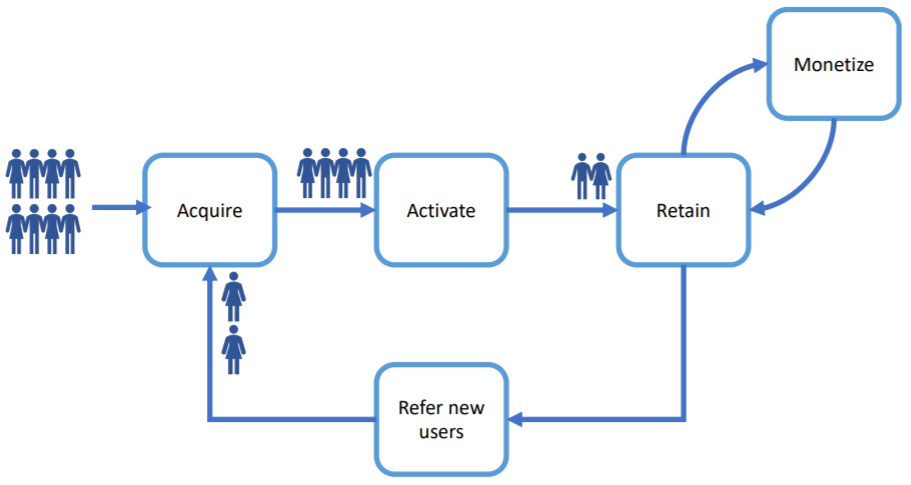
\includegraphics[scale=0.5]{src/18.6 User Journey.PNG}
\end{figure}
\noindent We use marketing techniques to acquire users. Then, we activate the users into a habit of using the product. Next, we retain the users. As long as the users are retained, we can monetise them. Moreover, they can refer the app the product to other users and acquire new users.

\section{Growth model}
We combine the compounding growth loops and the user journey optimisation to form the growth model. To get the initial set of users, we use linear marketing, e.g, search engine optimisation.

\section{Retention}
Retention is a very important part of the user journey. It is when we can monetise the user and acquire more users. Moreover, retention is the foundation of compounding growth.

We consider this with an example. Below is the graph of interest index over time for FarmVille.
\begin{figure}[H]
    \centering
    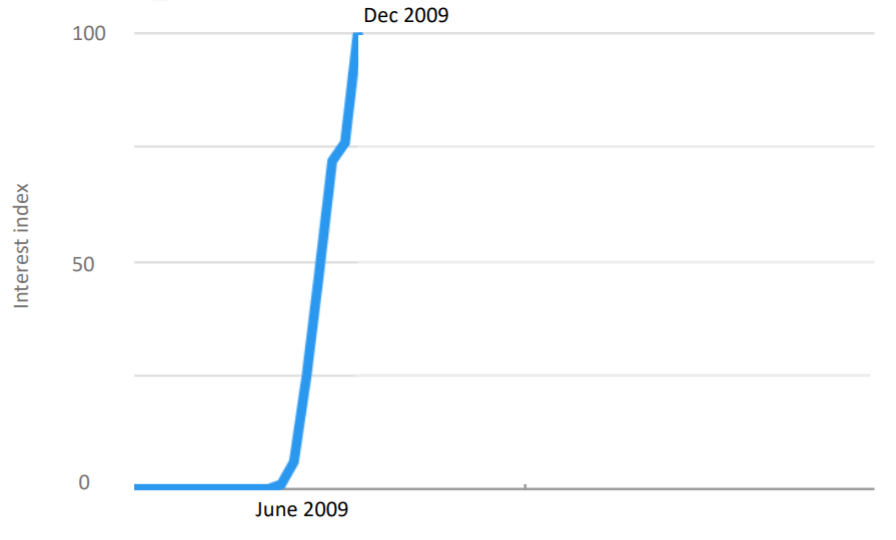
\includegraphics[scale=0.5]{src/18.7 FarmVille interest index (pre-fall).PNG}
\end{figure}
\noindent Although the trend until Dec 2009 is high, the product usage collapsed afterwards.
\begin{figure}[H]
    \centering
    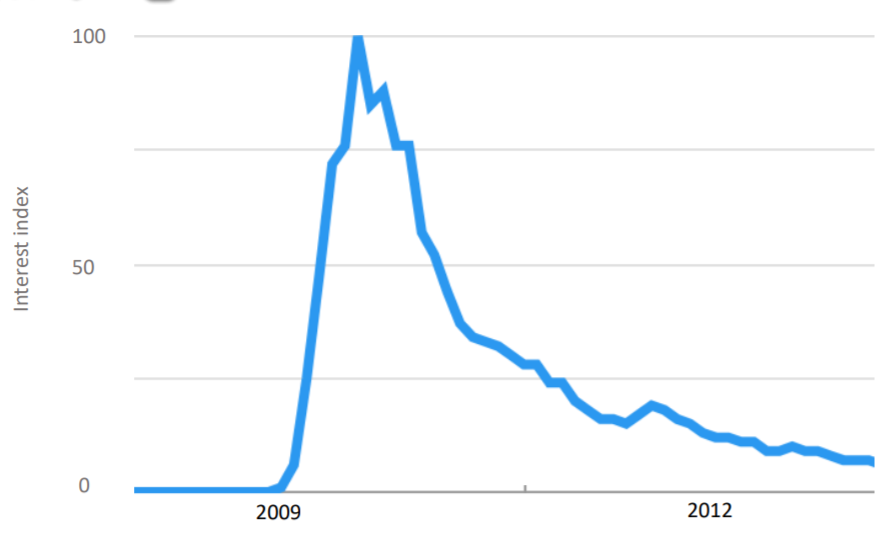
\includegraphics[scale=0.5]{src/18.8 FarmVille interest index (complete).PNG}
\end{figure}
\noindent To be able to predict whether the interest index is going to increase or decrease, we consider Retention-Cohort graphs.

Before that, we will look at some different possible churns for a software project. The following is a graph for a software project with zero churn.
\begin{figure}[H]
    \centering
    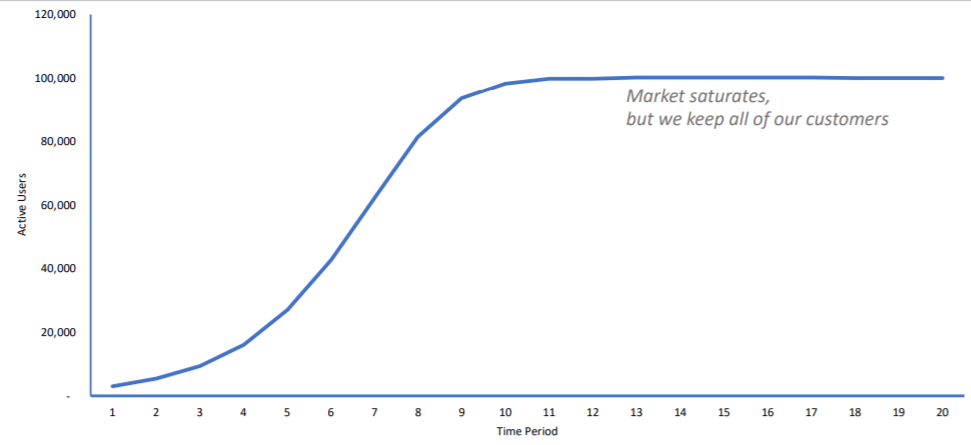
\includegraphics[scale=0.55]{src/18.11 0 Churn.PNG}
\end{figure}
\noindent The graph compares the number of active users with respect to the time period. Zero churn means that we retain all the users after acquisition. Users keep using the product, but because there is a limit to the number of users, the market saturates. For this reason, the graph goes flat after a point.

If we have 1\% churn, we get the following graph.
\begin{figure}[H]
    \centering
    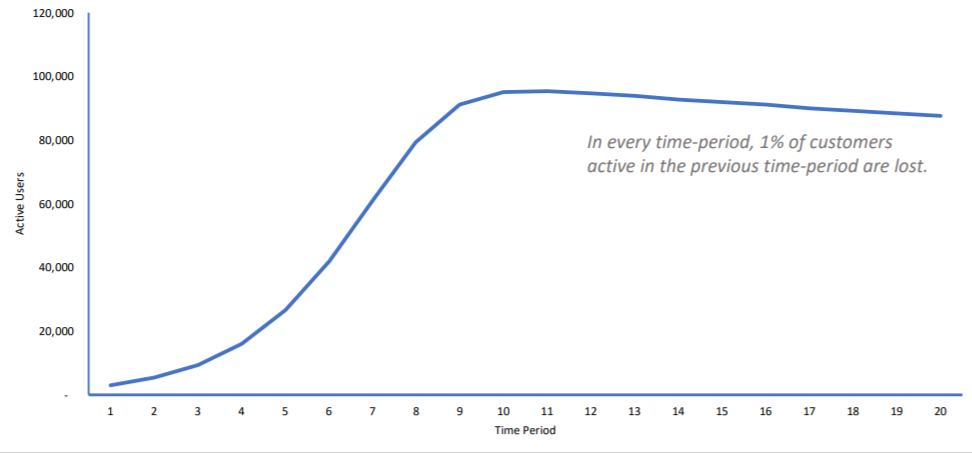
\includegraphics[scale=0.55]{src/18.12 1 Churn.PNG}
\end{figure}
\noindent 1\% churn means that 1\% of the users that use the product at a given time will stop using it later. This model is not the worst- it gives us plenty of time to improve the software so that we retain the customers.

Now, if we have 33\% churn, we get the following graph.
\begin{figure}[H]
    \centering
    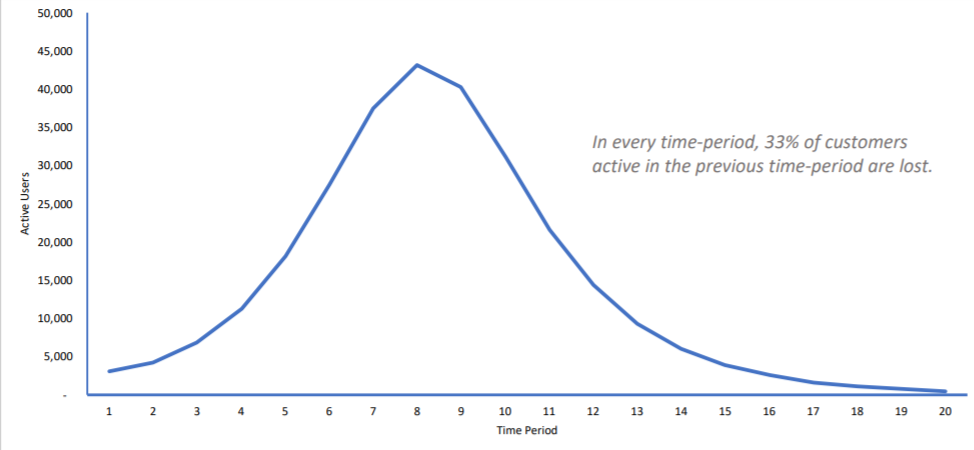
\includegraphics[scale=0.55]{src/18.13 33 Churn.PNG}
\end{figure}
\noindent This phenomenon is what we saw for FarmVille above. This is a jump the shark graph. This shows the importance of retention- although we are acquiring users at a good rate at the start, it is very important to have a high retention.

To see if the decline is predictable, we will consider the retention for a given cohort of users. Every user in a given cohort was acquired around the same time.
\begin{figure}[H]
    \centering
    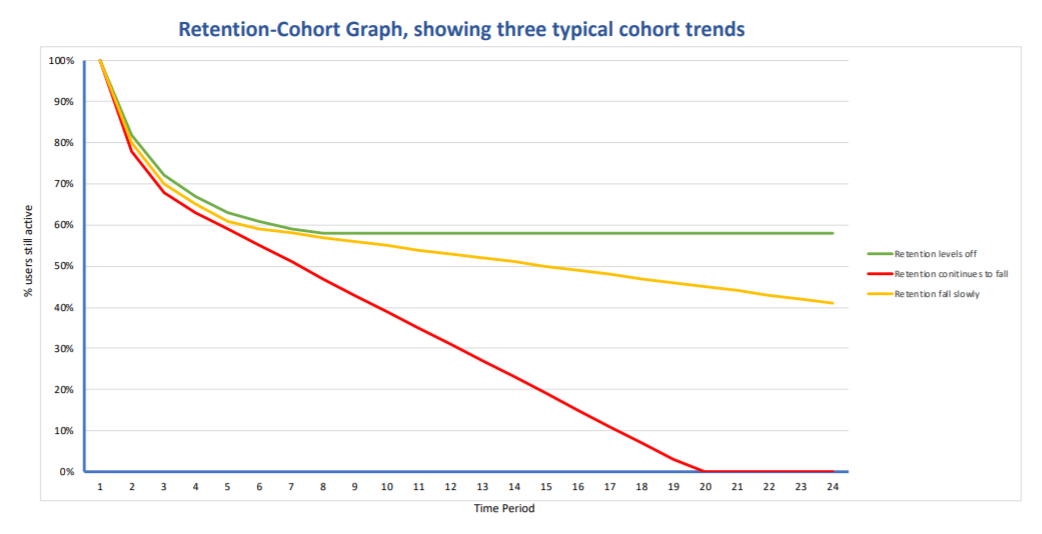
\includegraphics[scale=0.5]{src/18.14 Retention Cohort Graph.PNG}
\end{figure}
\noindent This is a retention-cohort graph. Here, we compare the number of active users after a given time period since acquisition.

The 3 lines illustrate the 3 possible outcomes for a cohort.
\begin{itemize}
    \item The green line represents the situation where we lose some users during the activation phase, but all the users are kept during the retention phase. This is a viable business.
    \item The yellow line represents the situation where we lose users during both the activation and the retention phase. If we make no changes, it is likely that the product will fail. Nonetheless, the decline during the retention phase is not very fast, so we still have time to stop the product from failing. The business model needs to be changed but it is not bad.
    \item The red line represents the situation where we lose users during both the activation and the retention phase. Moreover, the retention is very poor, and if there are many cohorts following this pattern, we get the jump in the shark graph. We need to drastically change the business model to stay in business.
\end{itemize}

In fact, we can loosely correspond the churns to the retention-cohort graphs. Zero churn represents the green line; 1\% churn represents the yellow line; and 33\% churn represents the red line.

It is important to highlight that retention is a trend and not a number. For example, we can have retention of 80\% in 4 weeks and 50\% in 12 weeks, but the cohort-retention graph could be the following.
\begin{figure}[H]
    \centering
    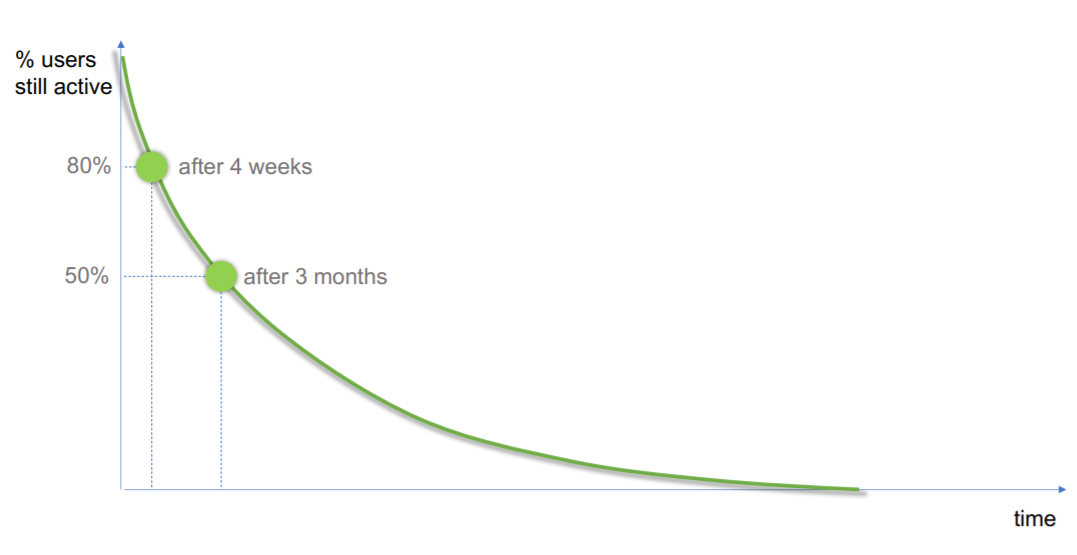
\includegraphics[scale=0.45]{src/18.15 Retention Trend v Retention Isolated Points.PNG}
\end{figure}
\noindent It is very important to see the trend. Single data points are not enough to determine the trend.

The cohort-retention graph can be broken into two phases of user journey-activation and retention. The activation phase takes place at the start, as shown below.
\begin{figure}[H]
    \centering
    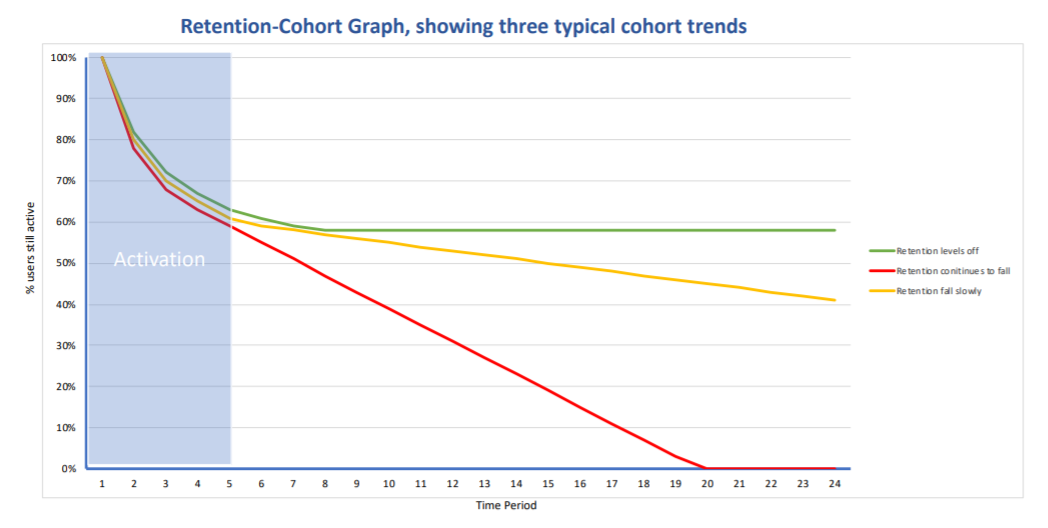
\includegraphics[scale=0.45]{src/18.16 Retention-Cohort Graph Activation Phase.PNG}
\end{figure}
\noindent After the activation phase has completed, we get the retention phase.
\begin{figure}[H]
    \centering
    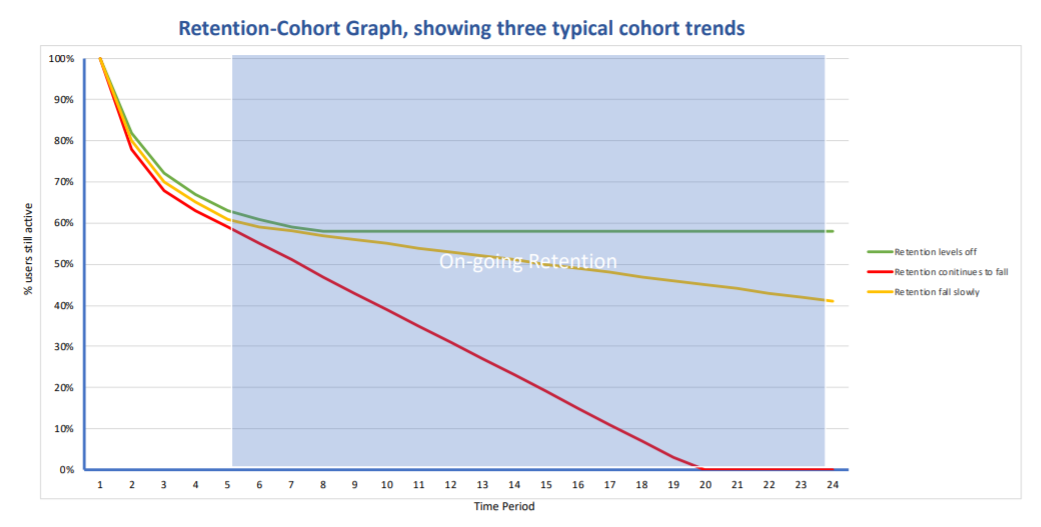
\includegraphics[scale=0.45]{src/18.17 Retention-Cohort Graph Retention Phase.PNG}
\end{figure}

Start-up teams make use of the growth model in the following way:
\begin{itemize}
    \item They generate hypotheses as to how the model could be improved (e.g. what could be done differently to improve activation).
    \item They prioritise their hypotheses based on how likely each hypothesis is to have the required outcome and how easy it is to implement it.
    \item They test some of the high-priority hypotheses.
    \item They learn from the results and make appropriate changes to the model.
\end{itemize}
This is a cycle, so we return back to the first stage. This process helps optimise activation and retention.

\section{Optimising compounding growth loops}
We can optimise compounding growth loops using the same growth model we saw above. We will illustrate this with an example. Consider the following growth loop for LinkedIn.
\begin{figure}[H]
    \centering
    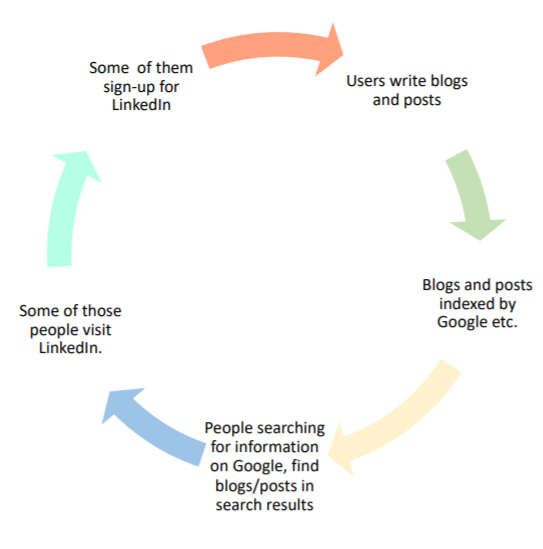
\includegraphics[scale=0.6]{src/18.18 LinkedIn growth loop 3.PNG}
\end{figure}
\noindent Each step in this loop can be optimised in theory. Although, it is possibly easier to optimise some steps in comparison to the others.

Assume the following is the current state of the growth loop:
\begin{itemize}
    \item We have 1 000 new users sign up for LinkedIn.
    \item About 10\% of them write a blog/post. So, 100 people create a new blog.
    \item We get about 100 clicks per month for each of those blogs. So, we get about 10 000 clicks.
    \item About 5\% of these people sign up for LinkedLin. So, we have 500 new sign ups from this cohort in a month.
\end{itemize}
There are many ways we could optimise this process. For example, we could have more pages with sign up buttons to recommend it, or make it more prominent. Similarly, we could make the page to write blogs more straightforward.

Using the growth model, we prioritise making it easier to write blogs and sign up. First, we prioritise making it easier to write blogs. This increases the proportion of users writing a blog from 10\% to 15\%. In that case, the state of the growth loop is:
\begin{itemize}
    \item We have 1 000 new users sign up for LinkedIn.
    \item About 15\% of them write a blog/post. So, 150 people create a blog.
    \item We get about 100 clicks per month for each of those blogs. So, we get about 15 000 clicks.
    \item About 5\% of these people sign up for LinkedIn. So, we have 750 new sign ups from this cohort in a month.
\end{itemize}
Next, if we also improve the sign up process, the proportion of users signing up increases from 5\% to 7.5\%. Then, state of the growth loop is:
\begin{itemize}
    \item We have 1 000 new users sign up for LinkedIn.
    \item About 15\% of them write a blog/post. So, 150 people create a blog.
    \item We get about 100 clicks per month for each of those blogs. So, we get about 15 000 clicks.
    \item About 7.5\% of these people sign up for LinkedIn. So, we have 1 125 new sign ups from this cohort in a month.
\end{itemize}
We could even optimise the searching process using Google indexing, and further increase the number of users that sign up.

\end{document}